\section{Descriptive and Exploratory Analysis}
\label{sec:review-eda}
\subsection{National airline data}
\label{sec:o4-national-data}
The DGCA monthly airline statistics, available through \href{https://github.com/mkubicek/india-aviation-stats}{Marek Kubicek's GitHub repository}, record passenger counts, available seat-kilometres (ASK) and revenue passenger-kilometres (RPK) for each airline. The passenger records show how traffic is divided among airlines, while ASK and RPK describe offered capacity and passenger traffic.

\subsubsection{Passenger shares and concentration}
From the passenger counts, we calculate each ownership group's share. Figure~\ref{fig:o4-national-eda} shows the combined share of the two largest groups (CR2) and the gap between them.
\begin{mergedcontribution}{authorGoutham}
\begin{figure}[!htbp]
\centering
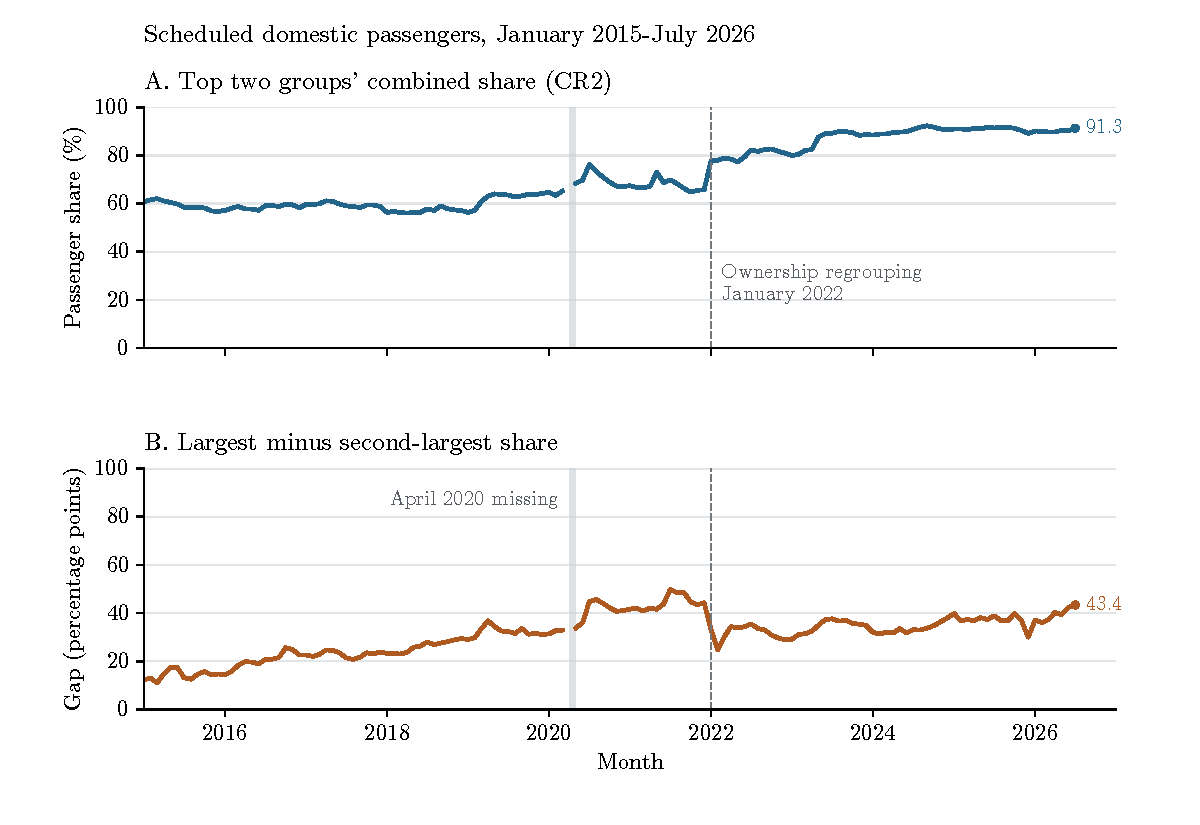
\includegraphics[width=\linewidth]{figures/o4_national_cr2_share_gap.pdf}
\caption{National concentration and share asymmetry, 2015--2026.}
\label{fig:o4-national-eda}
\vspace{2pt}
\begin{minipage}{\linewidth}
\footnotesize\setstretch{1.1}
\textit{Source:} DGCA monthly traffic via \href{https://github.com/mkubicek/india-aviation-stats/tree/16770ac59dae61ce7b80fd8bd67dd7f4cef280a6}{Kubicek (2026)}; authors' calculations.
\end{minipage}
\end{figure}

CR2 rises from 60.7\% to 91.3\% between January 2015 and July 2026, while the gap rises from 12.5 to 43.4 percentage points. IndiGo leads throughout, but the second-largest group changes (Appendix~\ref{app:o4-national-summary}). The January 2022 rise partly reflects the Tata Group's acquisition of Air India.


\end{mergedcontribution}
Period averages are reported in Appendix~\ref{app:eda-national-inputs}, Table~\ref{tab:o1-periods}.

\subsubsection{Changes around exits and entry}
\begin{mergedcontribution}{authorMeena}
A closer look at the exit windows shows that shares were already shifting before either airline stopped flying (Figure~\ref{fig:o2-exits}). Jet Airways' share fell from 16.2\% to 5.7\% in the year before its April 2019 exit, and Go First's from 11.1\% to 6.4\% before its May 2023 exit, as both grounded aircraft. The before-window therefore includes part of the shift and the comparison may understate it. IndiGo rose most around both exits, from about 43\% to 48\% after Jet Airways and from about 57\% to 62\% after Go First.

\begin{figure}[!htbp]
\centering
\color{authorMeena}
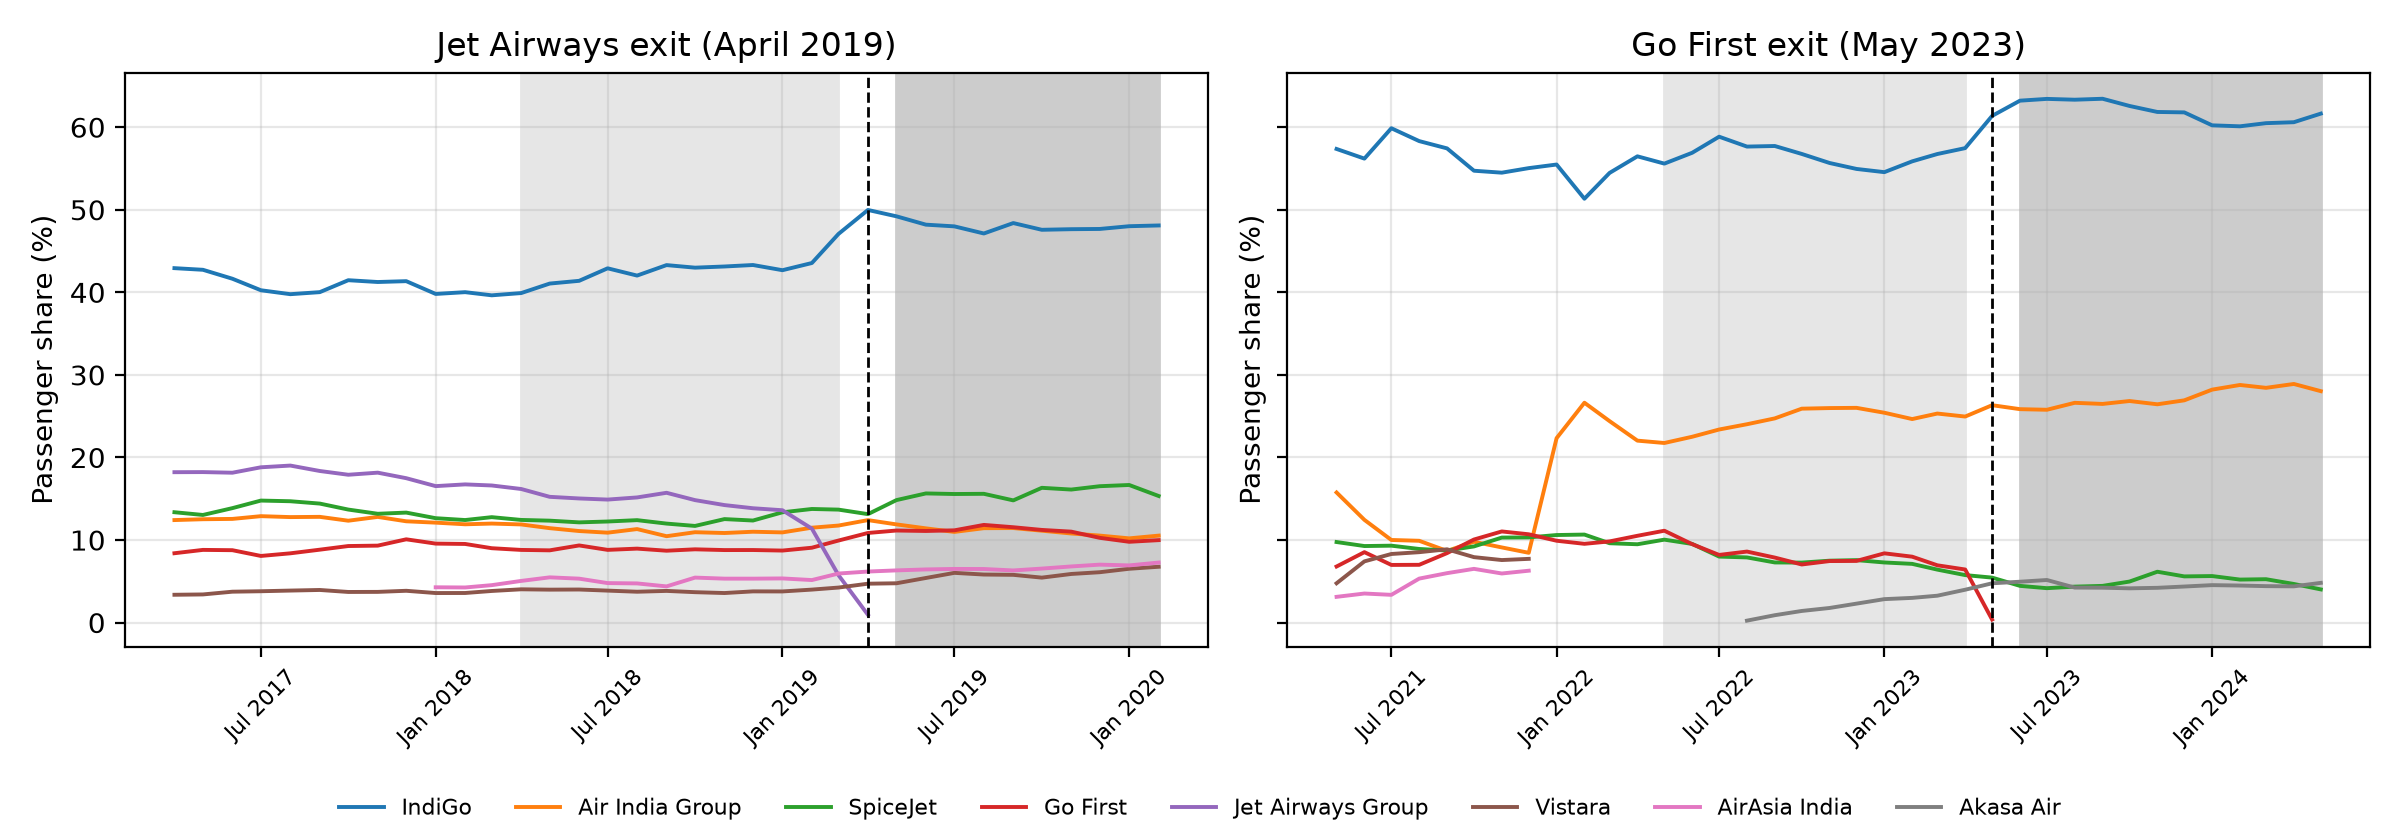
\includegraphics[width=\textwidth]{o2_exit_share_paths.png}
\caption{Monthly passenger shares by ownership group around the Jet Airways and Go First exits}\label{fig:o2-exits}
\sourcenote{DGCA monthly airline statistics via \textcite{kubicek2026aviationstats}; authors' calculations. Light shading: 12-month pre-exit window; dark shading: post-exit window (10 months for Jet Airways, ending before COVID-19); dashed line: exit month, excluded from both windows. The Air India Group's jump in January 2022 is the Tata acquisition grouping, not an exit effect.}
\end{figure}
\end{mergedcontribution}
Pre-consolidation Tata brand shares are in Appendix~\ref{app:eda-national-inputs}, Table~\ref{tab:o2-tata}.
\begin{mergedcontribution}{authorSweta}
Alongside these exits, nine entrants appear in the traffic records. Their peak passenger shares range from 0.01\% for Air Deccan to 10.44\% for Vistara, with different operating spans and outcomes (Figure~\ref{fig:o3-life}, Appendix~\ref{app:eda-entrant-spans}).
\end{mergedcontribution}
\subsubsection{Offered capacity and passenger traffic}
ASK and RPK allow us to compare the capacity offered with the passenger traffic carried. Market totals around the exits are in Appendix~\ref{app:eda-national-inputs}, Table~\ref{tab:o2-market}. The December capacity and passenger-traffic inputs are in Table~\ref{tab:o4-capacity-buffer}.

\subsection{DGCA approved flight schedules}
\label{sec:o4-route-data}
The national totals pool all routes. DGCA approved schedules give a closer view of individual airport pairs. Appendix~\ref{app:eda-route-support}, Table~\ref{tab:review-route-samples}, distinguishes the entrant and ownership-group samples.
\begin{mergedcontribution}{authorGoutham}
\begin{figure}[H]
\centering
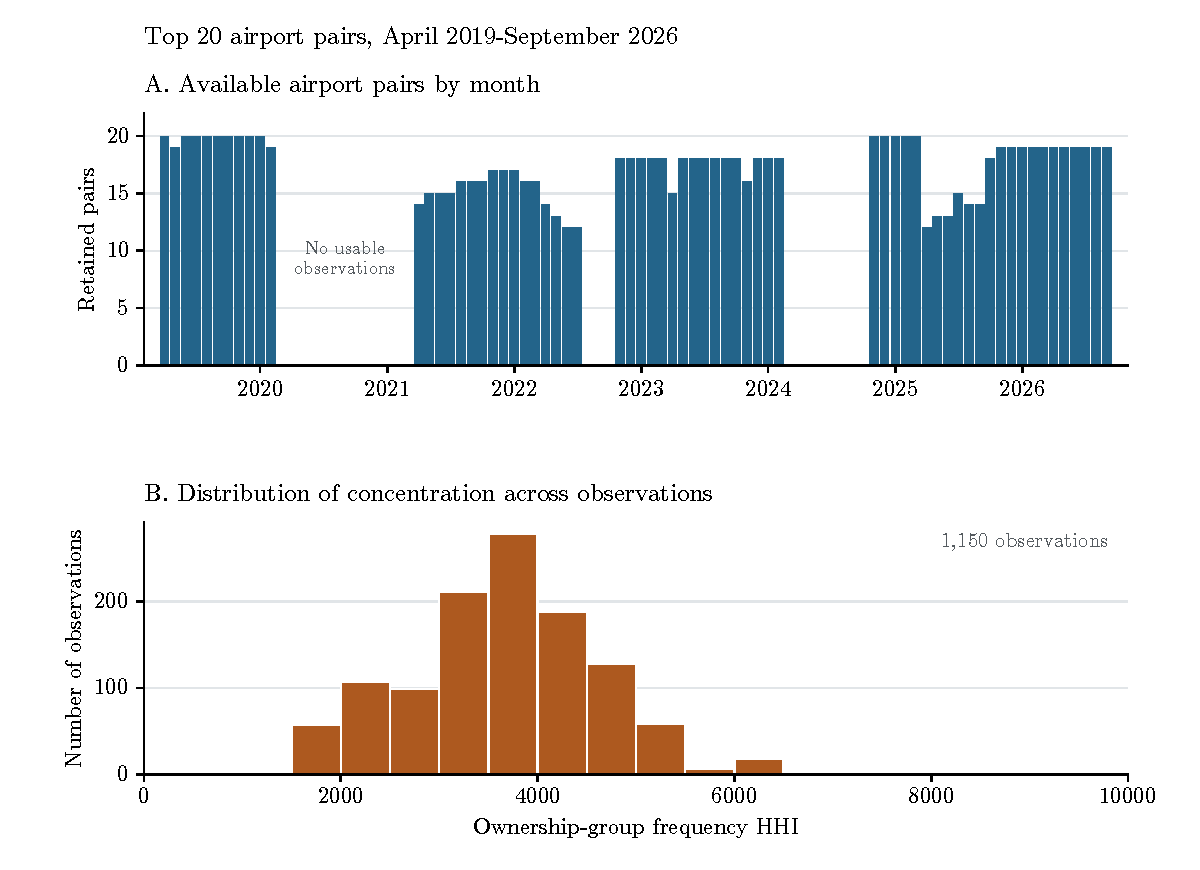
\includegraphics[width=\linewidth]{figures/o4_route_coverage_hhi.pdf}
\caption{Route-data coverage and the distribution of ownership-group frequency HHI.}
\label{fig:o4-route-eda}
\vspace{2pt}
\begin{minipage}{\linewidth}
\footnotesize\setstretch{1.1}
\textit{Source:} DGCA approved domestic schedules; authors' calculations.
\end{minipage}
\end{figure}
\end{mergedcontribution}
\begin{mergedcontribution}{authorSweta}
The entrant sample counts all scheduled departures in each airline's selected summer or winter season, including services that start or finish partway through it. It contains 229 records for nine entrants, with one record for each airline on each airport pair in its selected season. Monthly route records are analysed separately.
\end{mergedcontribution}
\begin{mergedcontribution}{authorGoutham}


Coverage ranges from 12 to 20 airport pairs per observed month. Median ownership-group HHI is 3,711, with the middle half between 3,180 and 4,244 (Figure~\ref{fig:o4-route-eda}). The histogram pools observations across airport pairs and months. Coverage gaps indicate unavailable data. Figure~\ref{fig:o4-route-heatmap} in Appendix~\ref{app:eda-route-support} shows individual airport pairs over time.
\end{mergedcontribution}
\subsection{Company financial and regulatory records}
\begin{mergedcontribution}{authorSweta}
Company and regulatory records add financial context to the entrant traffic patterns. Coverage differs across airlines and years. Net and operating results are kept separate. Missing financial figures are marked ``n.a.'' and left out of calculations that require them. Appendix~\ref{app:eda-financial-coverage}, Table~\ref{tab:review-financial-coverage}, records the coverage and accounting bases.
\end{mergedcontribution}
